\section{Implémentation de l'application web \\ \texttt{cognitivefactory-interactive-clustering-gui}}
\label{annex:C.4-DESCRIPTION-IMPLEMENTATION-INTERACTIVE-CLUSTERING-GUI}

	% INTRODUCTION DE L'ANNEXE.
	Au cours de ce doctorat, nous avons implémenté notre méthodologie de \textit{clustering} interactif au sein d'une application web.
	Celle-ci dispose de plusieurs fonctionnalités telles que :
	\begin{itemize}
		\item la gestion du projet, de ses données et de ses paramétrages ;
		\item la gestion et l'annotation de contraintes, ainsi que la vérification des propriétés de transitivités ;
		\item la gestion des étapes d'une itération de la méthode ;
		\item l'exécution asynchrone des divers algorithmes de la méthode (prétraitement, vectorisation, clustering, échantillonnage) ;
		\item quelques scripts d'analyses.
			% \footnote{Les scripts d'analyses concernent la visualisation des clusters et des composants connexes au cours des itérations, la vérification de la pertinence avec l'analyse des patterns linguistiques et les résumés automatiques de thématique, et l'analyse de la rentabilité avec l'évolution de la similarité entre résultats de \textit{clustering}.}.
	\end{itemize}
	
	Nous présenterons succinctement cette application ci-dessous à l'aide de captures d'écrans.
	
	% Information : comme y accéder.
	\begin{leftBarInformation}
		L'application est accessible dans \cite{schild-etal:2022:cognitivefactory-interactiveclusteringgui}.
		La documentation technique est accessible au lien suivant : \url{https://cognitivefactory.github.io/interactive-clustering-gui/}.
	\end{leftBarInformation}
	
	% Note de l'auteur : en cours de maintenance.
	\begin{leftBarAuthorOpinion}
		Suite aux diverses études menées au cours de ce doctorat, certaines pages sont en cours de refonte, notamment les pages d'analyses (suite aux conclusions des \textsc{Section~\ref{section:4.4-HYPOTHESE-PERTINENCE}} et \textsc{Section~\ref{section:4.5-HYPOTHESE-RENTABILITE}}) et les pages de documentations (suite à discussion en \textsc{Chapitre~\ref{chapter:5-GUIDE}}.
	\end{leftBarAuthorOpinion}
	
	
	%%% Page d'accueil de l'application
	\newpage
	\paragraph{Page d'accueil de l'application (\textsc{Figure~\ref{figure:C-WEB-APPLICATION-ACCUEIL}}) :}
		C'est la page de bienvenu de l'application.
		Nous y trouvons une description rapide de la méthode ainsi qu'une liste des questions fréquentes à son sujet.
		Le bouton en haut à gauche permettra toujours de revenir sur cette page.
		
		% Capture d'écran: Page d'accueil de l'application.
		\begin{figure}[H]
			\centering
			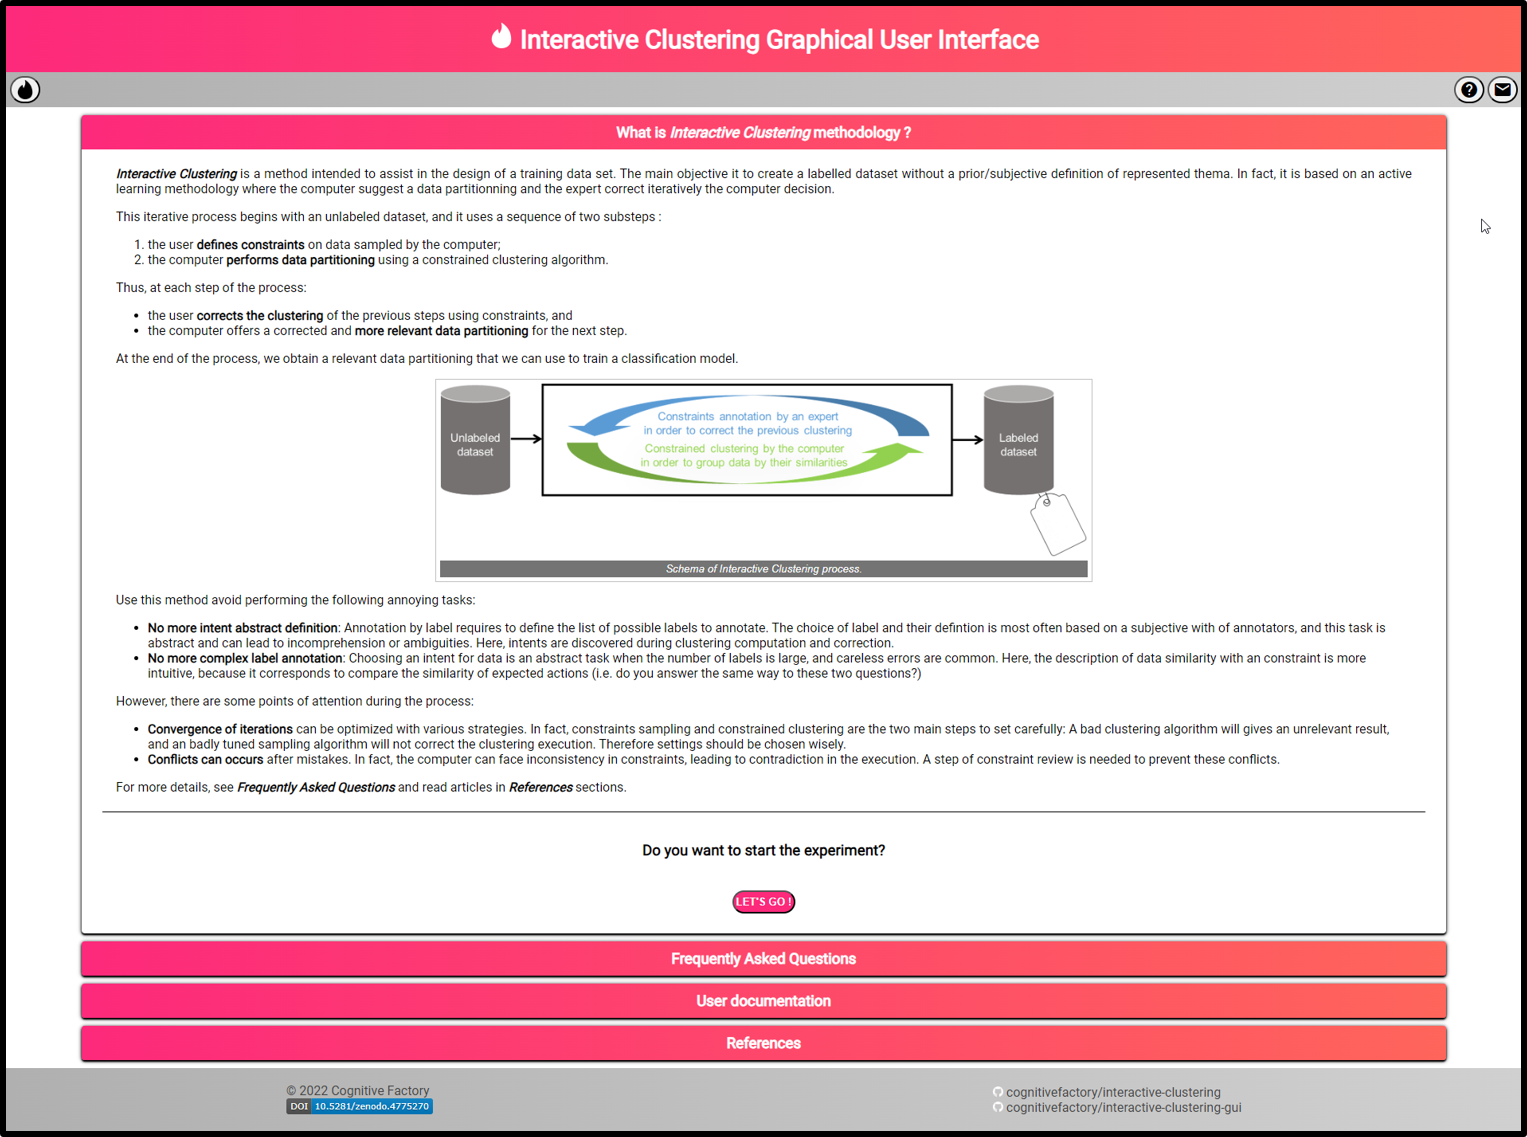
\includegraphics[width=0.95\textwidth]{figures/interactive-clustering-application-accueil-application}
			\caption{
				Capture d'écran de l'application web implémentant notre méthodologie de \textit{clustering} interactif : \textbf{page d'accueil de l'application}.
			}
			\label{figure:C-WEB-APPLICATION-ACCUEIL}
		\end{figure}
	
	
	%%% Page de gestion des projets
	\newpage
	\paragraph{Page de gestion des projets (\textsc{Figure~\ref{figure:C-WEB-APPLICATION-LISTE-PROJETS}}) :}
		Cette page liste les projets existants sous la forme de tuiles contenant les informations importantes : nom, date de création, nombre d'itérations de la méthode, et statut du projet (nous y reviendrons plus tard).
		Il est possible de télécharger un projet au format \texttt{.zip} ou de le supprimer.
		Pour créer un projet, le bouton \texttt{ADD NEW} ouvre un petit formulaire demandant le nom du projet et la liste des textes à annoter (au format \texttt{.csv} séparateur '\texttt{;}').
		Il est aussi possible d'importer un projet à l'aide d'une archive \texttt{.zip} téléchargée au préalable.
		Le bouton \texttt{LOAD} mène à la page d'accueil du projet sélectionné.
		
		% Capture d'écran: liste des projets.
		\begin{figure}[H]
			\centering
			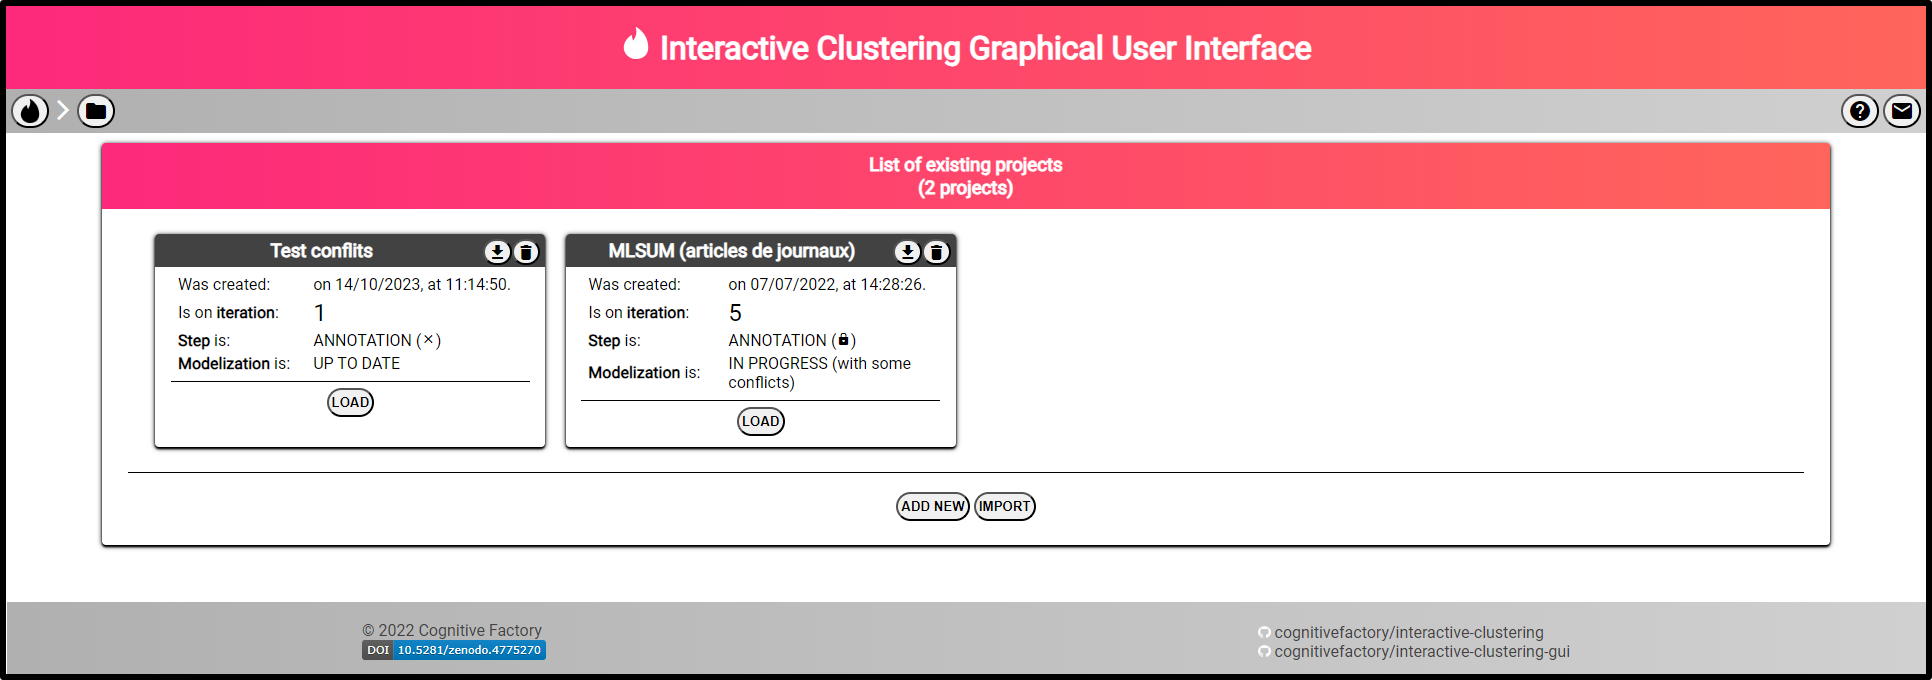
\includegraphics[width=0.95\textwidth]{figures/interactive-clustering-application-liste-projets}
			\caption{
				Capture d'écran de l'application web implémentant notre méthodologie de \textit{clustering} interactif : \textbf{page de gestion des projets}.
			}
			\label{figure:C-WEB-APPLICATION-LISTE-PROJETS}
		\end{figure}
	
	
	%%% Page d'accueil du projet en cours
	\newpage
	\paragraph{Page d'accueil du projet en cours (\textsc{Figure~\ref{figure:C-WEB-APPLICATION-ACCUEIL-PROJET}}) :}
		\todo[inline]{à rédiger}
	
		% Capture d'écran: accueil projet.
		\begin{figure}[H]
			\centering
			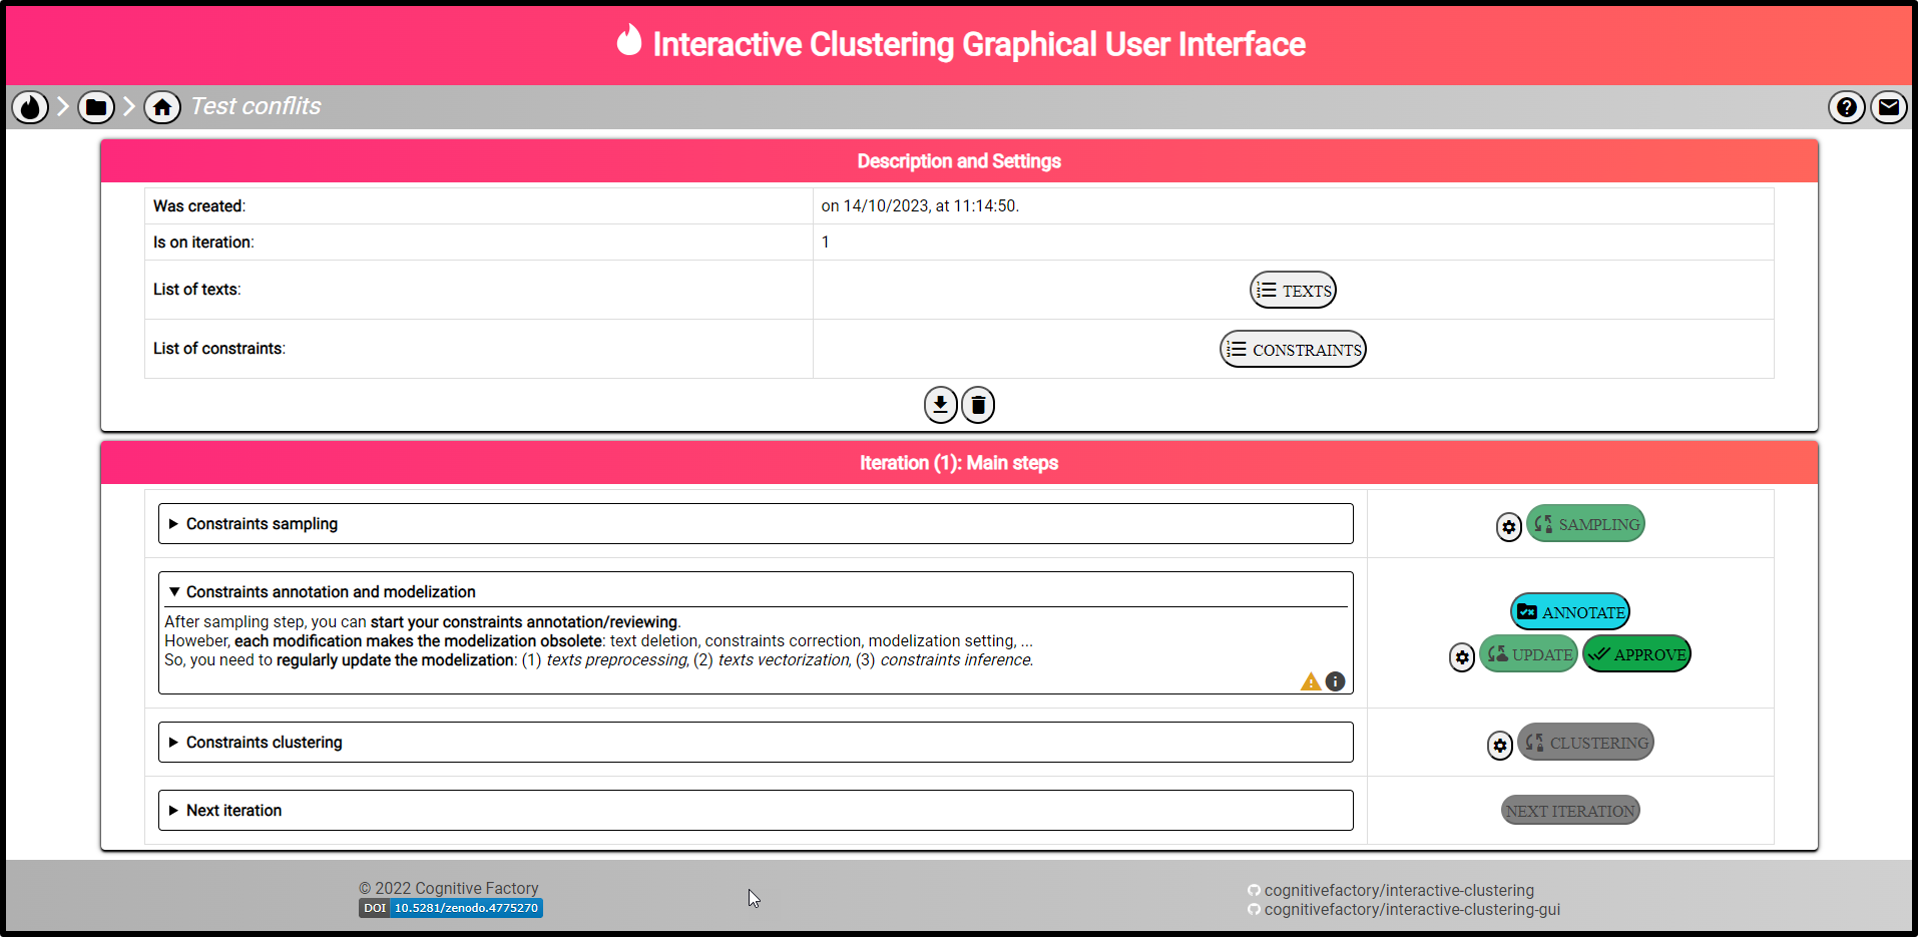
\includegraphics[width=0.95\textwidth]{figures/interactive-clustering-application-accueil-projet}
			\caption{
				Capture d'écran de l'application web implémentant notre méthodologie de \textit{clustering} interactif : \textbf{page d'accueil du projet en cours}.
			}
			\label{figure:C-WEB-APPLICATION-ACCUEIL-PROJET}
		\end{figure}
	
	
	%%% Diagramme d'états de l'application et gestion des exécutions asynchrones
	\newpage
	\paragraph{Diagramme d'états de l'application et gestion des exécutions asynchrones (\textsc{Figure~\ref{figure:C-WEB-APPLICATION-DIAGRAMME-ETATS}}) :}
		\todo[inline]{à rédiger}
	
		% Capture d'écran: accueil projet.
		\begin{figure}[H]
			\centering
			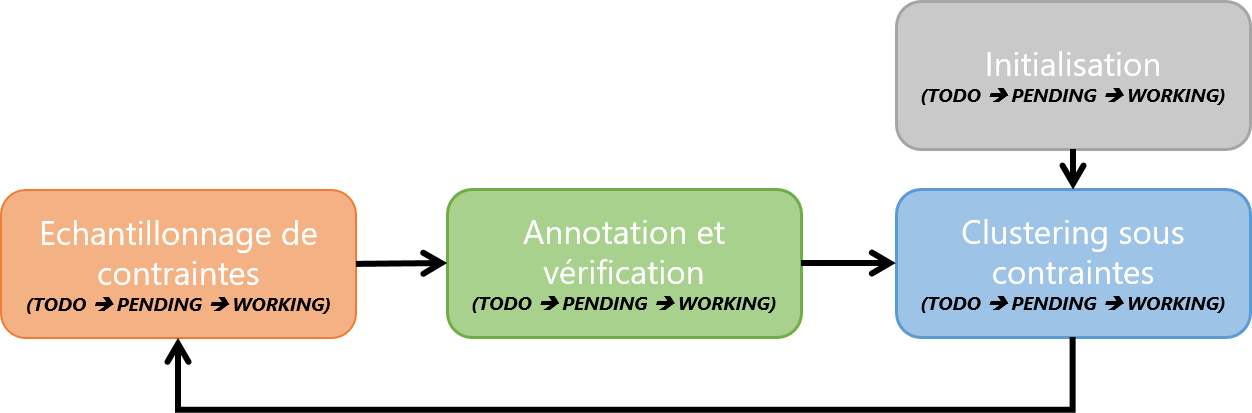
\includegraphics[width=0.95\textwidth]{figures/interactive-clustering-application-diagramme-etats}
			\caption{
				\textbf{Diagramme d'états} simplifié de l'application web implémentant notre méthodologie de \textit{clustering} interactif.
			}
			\label{figure:C-WEB-APPLICATION-DIAGRAMME-ETATS}
		\end{figure}
	
	
	%%% Page de gestion des paramètres
	\newpage
	\paragraph{Page de gestion des paramètres (\textsc{Figure~\ref{figure:C-WEB-APPLICATION-PARAMETRAGE}}) :}
		\todo[inline]{à rédiger}
	
		% Capture d'écran: gestion des paramètrages.
		\begin{figure}[H]
			\centering
			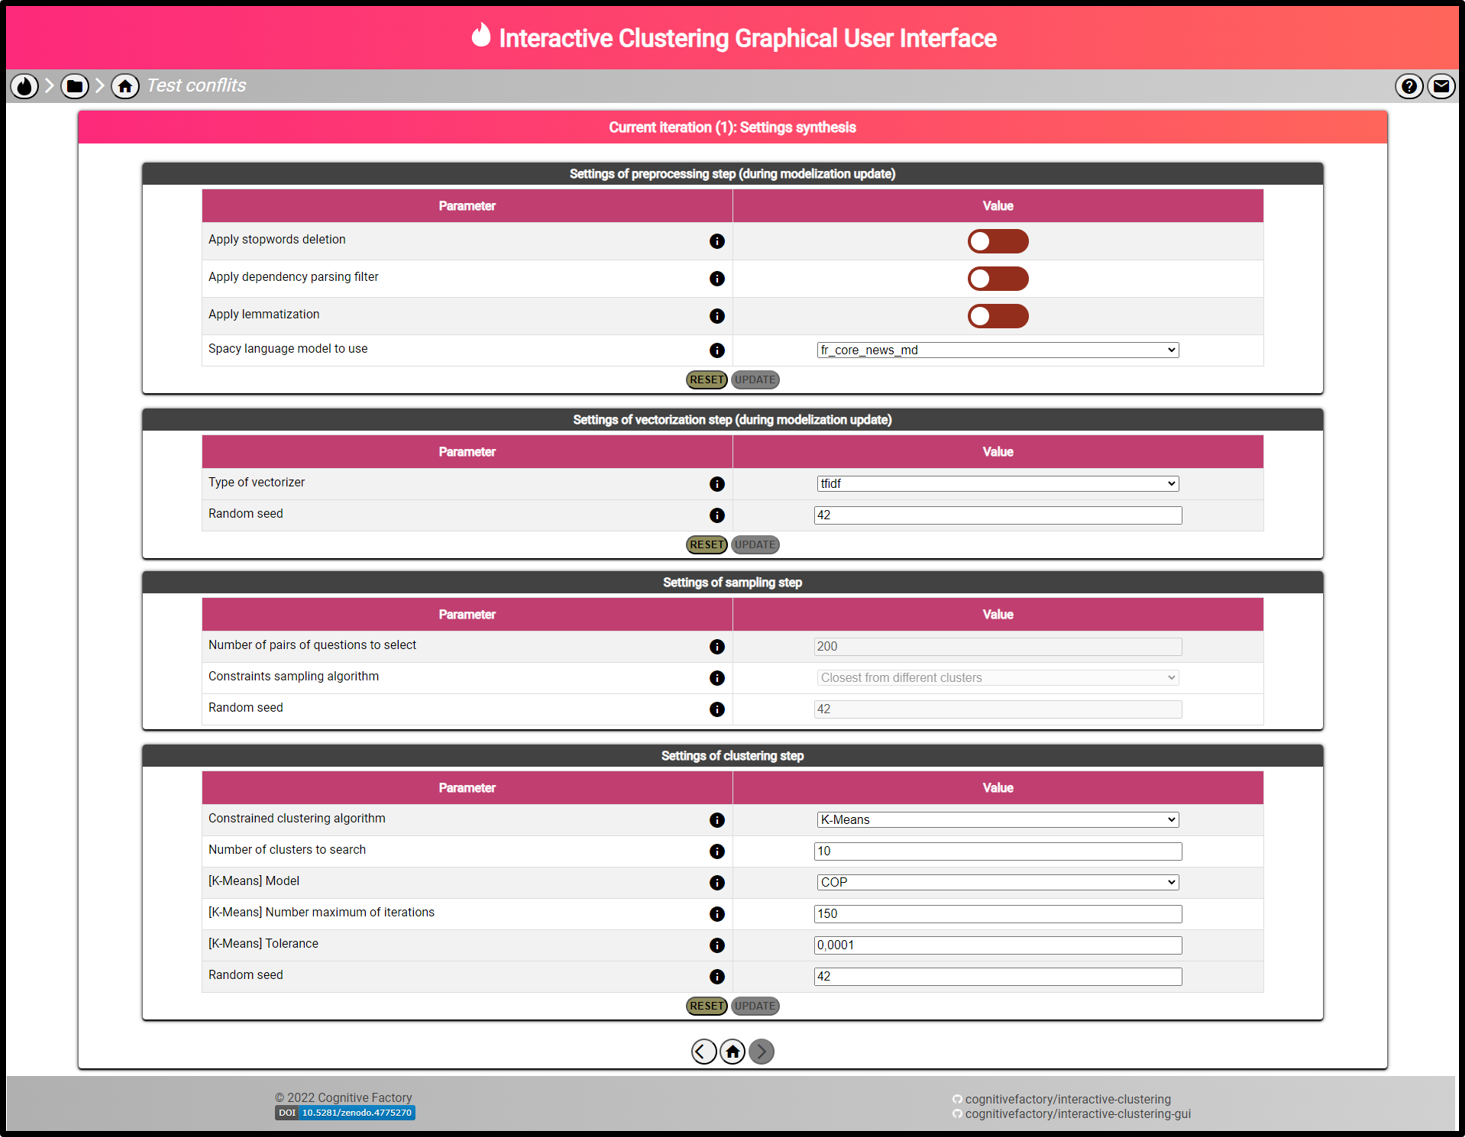
\includegraphics[width=0.95\textwidth]{figures/interactive-clustering-application-parametres}
			\caption{
				Capture d'écran de l'application web implémentant notre méthodologie de \textit{clustering} interactif : \textbf{page de gestion des paramètres}.
			}
			\label{figure:C-WEB-APPLICATION-PARAMETRAGE}
		\end{figure}
	
	
	%%% Page d'inventaire des textes
	\newpage
	\paragraph{Page d'inventaire des textes (\textsc{Figure~\ref{figure:C-WEB-APPLICATION-INVENTAIRE-TEXTES}}) :}
		\todo[inline]{à rédiger}
	
		% Capture d'écran: inventaire des textes.
		\begin{figure}[H]
			\centering
			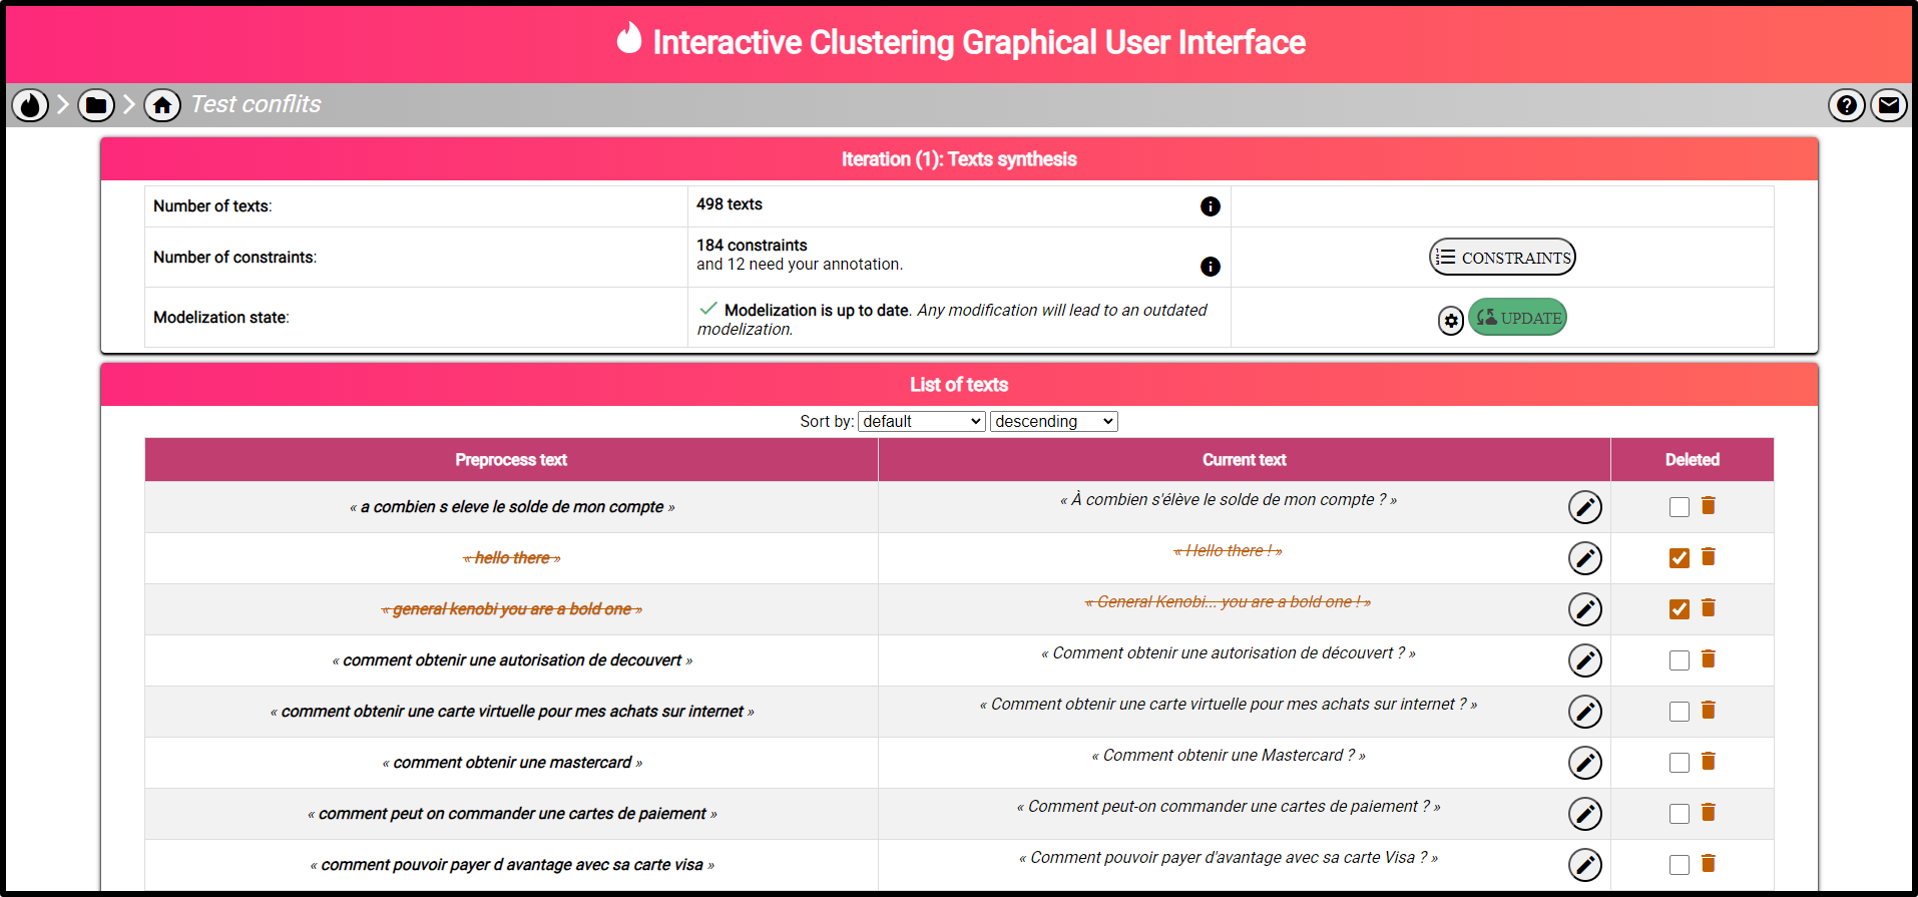
\includegraphics[width=0.95\textwidth]{figures/interactive-clustering-application-textes}
			\caption{
				Capture d'écran de l'application web implémentant notre méthodologie de \textit{clustering} interactif : \textbf{page d'inventaire des textes}.
			}
			\label{figure:C-WEB-APPLICATION-INVENTAIRE-TEXTES}
		\end{figure}
	
	
	%%% Page d'inventaire des contraintes
	\newpage
	\paragraph{Page d'inventaire des contraintes (\textsc{Figure~\ref{figure:C-WEB-APPLICATION-INVENTAIRE-CONTRAINTES}}) :}
		\todo[inline]{à rédiger}
	
		% Capture d'écran: inventaire des contraintes.
		\begin{figure}[H]
			\centering
			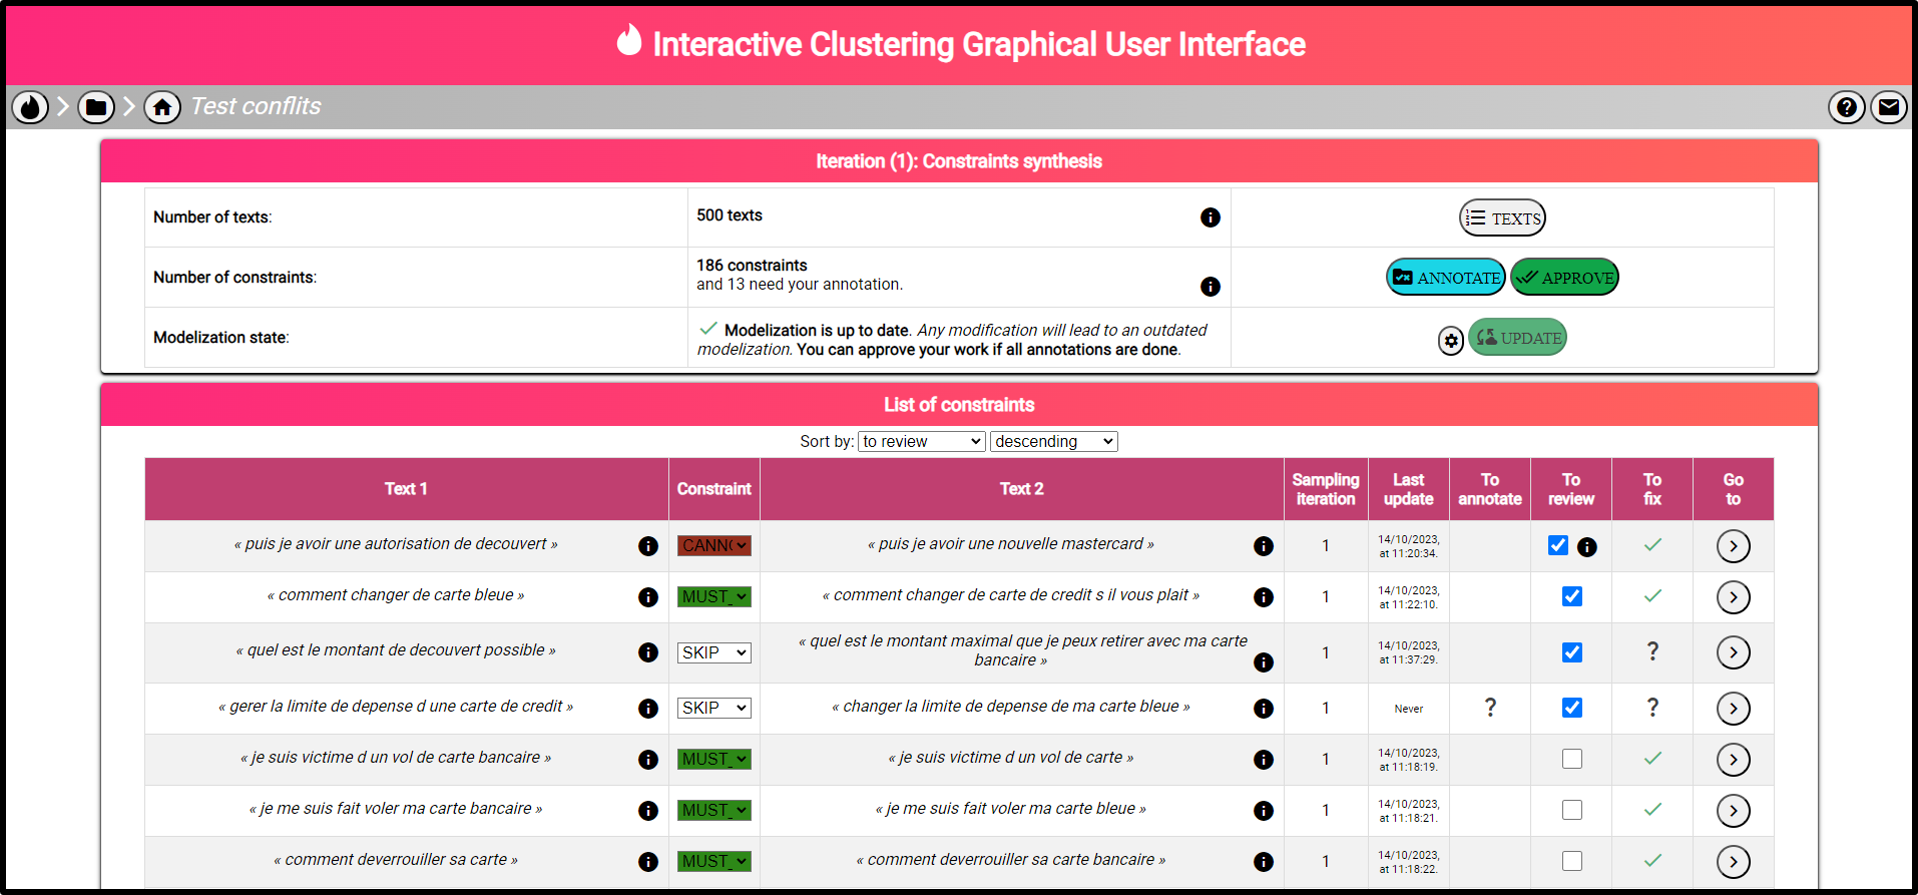
\includegraphics[width=0.95\textwidth]{figures/interactive-clustering-application-contraintes}
			\caption{
				Capture d'écran de l'application web implémentant notre méthodologie de \textit{clustering} interactif : \textbf{page d'inventaire des contraintes}.
			}
			\label{figure:C-WEB-APPLICATION-INVENTAIRE-CONTRAINTES}
		\end{figure}
	
	
	%%% Page d'annotation d'une contrainte
	\newpage
	\paragraph{Page d'annotation d'une contrainte (\textsc{Figure~\ref{figure:C-WEB-APPLICATION-ANNOTATION}} et \textsc{Figure~\ref{figure:C-WEB-APPLICATION-CONFLIT}}) :}
		\todo[inline]{à rédiger}
	
		% Capture d'écran: annotation.
		\begin{figure}[H]
			\centering
			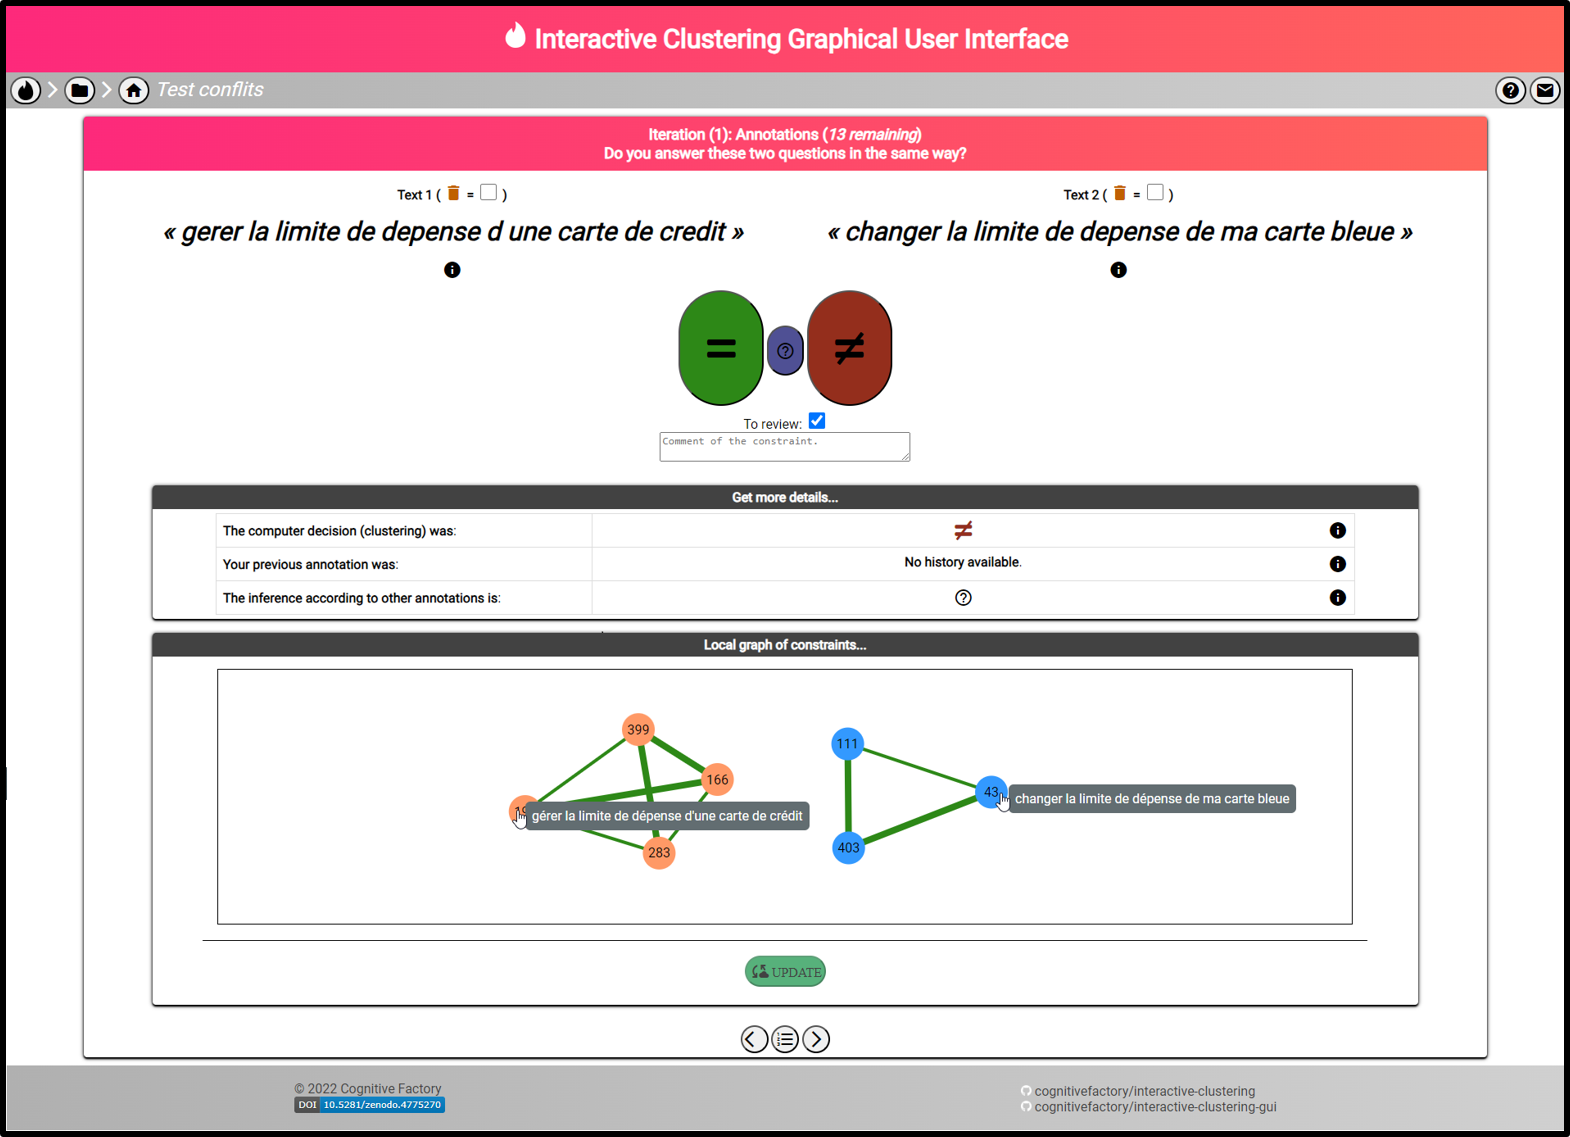
\includegraphics[width=0.95\textwidth]{figures/interactive-clustering-application-annotation-0full}
			\caption{
				Capture d'écran de l'application web implémentant notre méthodologie de \textit{clustering} interactif : \textbf{page d'annotation d'une contrainte}.
			}
			\label{figure:C-WEB-APPLICATION-ANNOTATION}
		\end{figure}
		
		% Capture d'écran: conflit d'annotation.
		\begin{figure}[H]
			\centering
			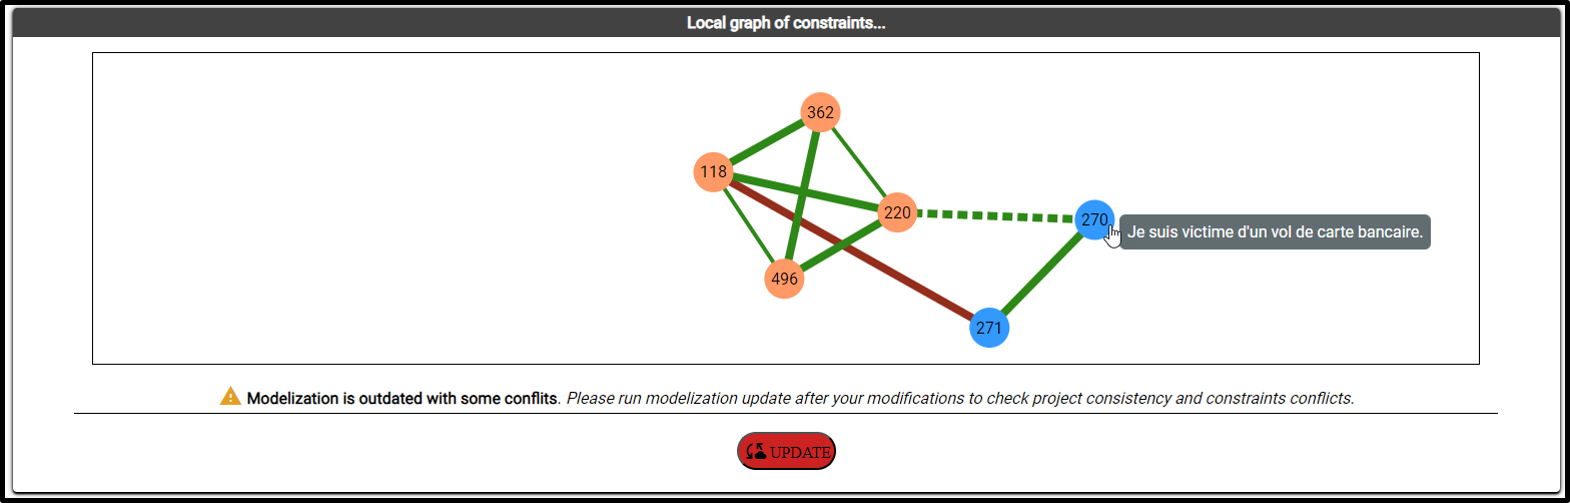
\includegraphics[width=0.95\textwidth]{figures/interactive-clustering-application-annotation-4conflit}
			\caption{
				Capture d'écran de l'application web implémentant notre méthodologie de \textit{clustering} interactif : \textbf{graphe de contraintes présentant un conflit d'annotation}.
			}
			\label{figure:C-WEB-APPLICATION-CONFLIT}
		\end{figure}